\documentclass{article}
\usepackage{graphicx}
\usepackage{amsmath}
\usepackage{acronym}
\usepackage{biblatex}

\title{Aposteriori Unimodality}
\author{Dimitris Tsirmpas, John Pavlopoulos}
\date{March 2025}


% Insert space after commas in math mode
\AtBeginDocument{%
  \mathchardef\stdcomma=\mathcode`,
  \mathcode`,="8000
}
\begingroup\lccode`~=`, \lowercase{\endgroup\def~}{\stdcomma\,}

\graphicspath{ {../graphs}  }
\bibliography{refs.bib}


\begin{document}

\maketitle

\section{Methodology}

\subsection{Problem Formulation}
\label{ssec:methodology:problem}

Let $\{c(d,1), c(d,2), \ldots\}$ be the comments\footnote{Also referred to as “dialogue turns” in some publications.} of a discussion $d$. We assume that annotating a comment depends on three variables: its contents, the annotator's \ac{SDB}, and uncontrolled factors such as mood and personal experiences. Assuming that each comment is assigned multiple annotators, we can define the annotation set $A(d, i)$ for comment $c(d, i)$ as:
\begin{equation}
    A(d, i) = \{a(d, i, \theta) \mid i=1, 2, \ldots, \lvert d \rvert, \theta \in \Theta \}
\end{equation}
\noindent where  $a(d, i, \theta)$ is a single annotation for comment $c(d,i)$ and $\Theta$ is the set of annotator \acp{SDB}.

Since our goal is to pinpoint which specific characteristics contribute to polarization, we need a way to isolate individual attributes within a \ac{SDB}. $\Theta$ is usually composed of multiple ``dimensions'' (e.g., age, sex, educational level), each of which is split between various groups. We can thus model $\theta \in \Theta$ as:
\begin{equation}
    \theta = \{(\xi_i, g) \mid i=1, 2, \ldots, k \mathpunct{,} g \in G_i\}
\end{equation} 
\noindent where $\Xi=\{\xi_1, \xi_2, \ldots, \xi_k\}$ is the set of \ac{SDB} dimensions, and $G_i$ is the set of possible groups for dimension $\xi_i$ (e.g., if $\xi_1$ corresponds to gender, then $G_1=\{\textit{male}, \textit{female}, \ldots\}$).


\subsection{Quantifying changes in polarization}
\label{ssec:methodology:polstat}

The mechanism defined in \S\ref{ssec:methodology:problem} allows us to isolate the effects of each \ac{SDB} dimension $\xi$, but we still lack a mechanism with which to analyze that effect. In this section, we present the "pol-statistic" (polarization statistic) as a comment-level tool which not only attributes polarization to a dimension $\xi$, but also to specific groups within that dimension $g \in G_{\xi}$.

Intuitively, dimension $\xi$ partially explains polarization when the annotations divided according to each group $g \in G_{\xi}$, show less polarization between each group compared to the full set of annotations. Figure~\ref{fig:ndfu_single_comment} exhibits a hypothetical example, where a misogynistic comment is annotated for toxicity by male and female annotators. The annotations are generally polarized ($nDFU_{all} = 0.625$), although the set of annotations from female annotators might exhibit low polarization between themselves ($nDFU_{women} = 0.100$---most agree the comment is toxic). The set of male annotations on the other hand, also shows low polarization ($nDFU_{men} = 0.3725$), but for the opposite reason---most men agree that it is \emph{not} toxic. This suggests that the overall polarization is driven by disagreements between male and female annotators. 

%TODO: Do I use 2 genders here?
%TODO: Use actual data in plot?
\begin{figure}[t]
	\centering
	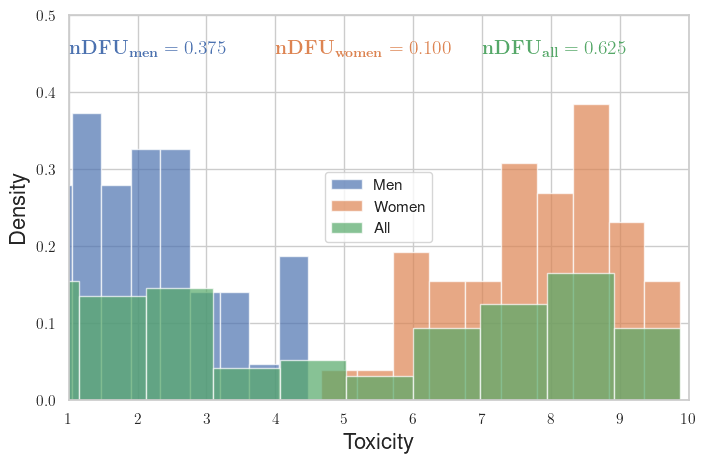
\includegraphics[width=0.8\linewidth]{ndfu_single_comment.png}
	\caption{Hypothetical example of a polarizing comment, where male and female annotators agree between themselves, but disagree with the opposite gender. Overall polarization ($nDFU_{all} = 0.625$) is much greater than the polarization exhibited by the annotations grouped by gender ($nDFU_{men} = 0.3725, nDFU_{women} = 0.100$). In this example, the annotation set $A$ was generated as $A_{men} \sim \mathcal{N}(2, 1.3), A_{women} \sim \mathcal{N}(8, 1.3), \lvert A_{men} \rvert = \lvert A_{women} \rvert = 50$.}
	\label{fig:ndfu_single_comment}
\end{figure}

% Intra group compared to inter-group?
 Given this observation, we would be tempted to aggregate all annotations for each comment in a discussion, and test whether intra-group polarization is greater than global polarization. However, this formulation would not work well, as illustrated in  Figure~\ref{fig:ndfu_multi_comment}. It features a hypothetical discussion with two comments, both of which are toxic, but where male and female annotators disagree on \emph{which} comment is the toxic one. If we aggregate the annotations for the two comments, the opposing polarization effects might balance each other out, leading to a false negative. In our example, while it is obvious that gender partly explains the polarization found in each of the individual comments ($nDFU_{all} \gg nDFU_{men}, nDFU_{all} \gg nDFU_{women}$), this observation is much harder to make when aggregating the two comments.
 
  To avoid this, we apply our statistic only on annotations that reference the same comment. Thus, we can define our ``pol-statistic" as:
\begin{equation}
	pol(c, \mu) = nDFU(A) - nDFU(P(A, \xi, g))
\end{equation}
\noindent where $P(A,\xi, g) = \{a(d, i, u) \in A | (\xi, \mu) \in \theta\}$ is the partition of $A$ for a comment $c(d, i)$ for which its annotators belong  to the group $g$ of \ac{SDB} dimension $\xi$.

\begin{figure}[t]
	\centering
	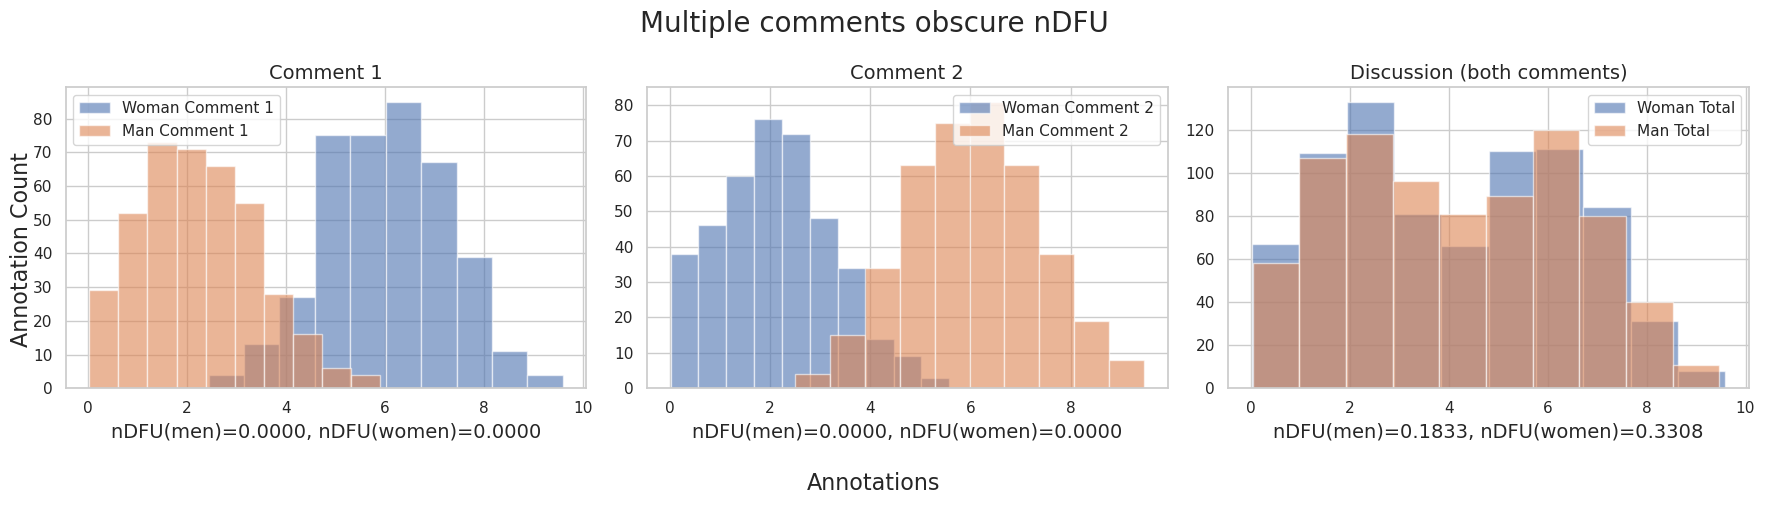
\includegraphics[width=\linewidth]{ndfu_multi_comments.png}
	\caption{Hypothetical example of a polarizing discussion with two comments, for which the annotators disagree which is the toxic one. If we aggregate the two comments, the polarization scores for both men and women significantly rise, obscuring whether the exhibited polarization can be partially attributed to gender. In this example, the annotation set $A$ was generated as $A_{men} \sim \mathcal{N}(6, 1), A_{women} \sim \mathcal{N}(2, 1), \lvert A_{men} \rvert = \lvert A_{women} \rvert = 200$ for the first comment, and $A_{men} \sim \mathcal{N}(2, 1), A_{women} \sim \mathcal{N}(6, 1), \lvert A_{men} \rvert = \lvert A_{women} \rvert = 200$ for the second.}
	\label{fig:ndfu_multi_comment}
\end{figure}



\subsection{The Aposteriori Unimodality Test}
\label{ssec:methodology:aposteriori}

Although intuitive, the \textit{pol statistic} can only be applied to individual comments, and is susceptible to inherent noise present in annotation tasks. If the polarization in a discussion $d$ is not driven by the attribute $\xi$, we would expect $pol(c, g) \approx 0,  \forall g \in G_{\xi}$. By obraining the pol statistics for all comments in a discussion $d$ we can apply a mean test with the null hypothesis :
\begin{equation}
	H_0: \frac{1}{\lvert d \rvert} \sum\limits_{c \in d} pol(c, g) = 0, \forall g \in G_{\xi}
\end{equation}
\noindent versus the alternative hypotheses: 
\begin{equation}
	H_i:  \frac{1}{\lvert d \rvert} \sum\limits_{c \in d}  pol(c, g_i) > 0, g_i \in G_{\xi}
\end{equation}

Since we are considering $\lvert G_{\xi} \rvert$ tests, we apply a multiple comparison correction to the resulting p-values. We choose the Bonferroni method \parencite{Bland170}, since it is widely used, generally conservative, and especially so towards correlated hypotheses \parencite{ChenFengYi2017}. The last point is important, since many annotation groups are likely to be inter-correlated (e.g., age categories such as 50-60 and 60-70 years). Furthermore, one of its biggest weaknesses (the presence of very large numbers of hypotheses \parencite{ChenFengYi2017}) is unlikely to be met in annotation tasks.

We refer to this test as the \textit{``Aposteriori Unimodality Test''}, where a small p-value suggests that we can not rule out that annotators of the $g$ group make a significant contribution to the overall annotator polarization.


\section{Acronyms}

\begin{acronym}[WWW]
    \acro{SDB}{SocioDemographic Background}
    \acro{nDFU}{normalized Distance From Unimodality}
\end{acronym}

\printbibliography

\end{document}
